\documentclass[tikz]{standalone}
\begin{document}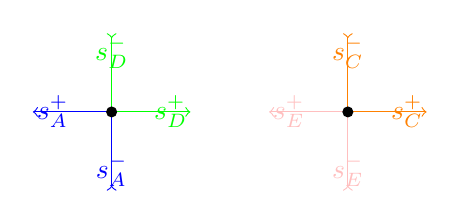
\begin{tikzpicture}

\draw[->,green] (0,0) -- node[near end] {$s_D^+$} (0:1);
\draw[-<,green] (0,0) -- node[near end] {$s_D^-$} (90:1);
\draw[->,blue] (0,0) -- node[near end] {$s_A^+$} (180:1);
\draw[-<,blue] (0,0) -- node[near end] {$s_A^-$} (270:1);
\fill[black] (0,0) circle (2pt);

\begin{scope}[xshift=3cm]
\draw[->,orange] (0,0) -- node[near end] {$s_C^+$} (0:1);
\draw[-<,orange] (0,0) -- node[near end] {$s_C^-$} (90:1);
\draw[->,pink] (0,0) -- node [near end] {$s_E^+$} (180:1);
\draw[-<,pink] (0,0) -- node [near end] {$s_E^-$} (270:1);
\fill[black] (0,0) circle (2pt);
\end{scope}

\end{tikzpicture}\end{document}
